\section{Introduction \& System overview}

%ML is a good alternative to computing the full analytical 
\Gls{ml} has emerged as a powerful paradigm for applications that rely on data-driven optimization, improving system performance by iteratively training on data. Following the introduction of the perceptron by \citeauthor{rosenblattPerceptron1958}, \citeauthor{rumelhartLearningRepresentationsBackpropagating1986} demonstrated that \gls{nn} with hidden layers, trained via backpropagation, can solve non-linearly separable problems such as the XOR problem \cite{rosenblattPerceptron1958,rumelhartLearningRepresentationsBackpropagating1986}. 
This laid the groundwork for a broad range of applications, ultimately enabling the era of transformer-based \cite{vaswaniAttentionAllYou2017} and generative AI models \cite{brownLanguageModelsAre2020a, radfordImprovingLanguageUnderstanding}. 
The performance of such deep-learning models was found to scale predictably as a power law with model size, dataset size, and training compute \cite{kaplanScalingLawsNeural2020, hoffmannTrainingComputeoptimalLarge2022}.
This scaling comes at a substantial energy cost: In 2025 data centers are estimated to account for 1.5\% of global electricity generation, driven increasingly by AI workloads \cite{OurWorldInData, samborskaScalingHowIncreasing2025}.

Photonic hardware offers a promising substrate for running neural networks more efficiently. \citeauthor{cybenkoApproximationSuperpositions1989} and \citeauthor{hornikMultilayerFeedforwardNetworks1989} showed in 1989 that neural networks can approximate any continuous function, given tunable weighted interconnections and non-linear activation functions \cite{cybenkoApproximationSuperpositions1989, hornikMultilayerFeedforwardNetworks1989}. 
Optical systems can provide both. 
As early as 1994, \citeauthor{reckExperimentalRealizationAny1994} demonstrated that any unitary operator can be realized with optical components, enabling arbitrary linear transformations in the optical domain \cite{reckExperimentalRealizationAny1994}. 
Among the various optical neural network (ONN) implementations proposed since, on-chip meshes of \glspl{mzi} stand out for their scalability
\cite{clementsOptimalDesignUniversal2016, shenDeepLearningCoherent2017}. 
Built from single-mode phase shifters and 50:50 beam splitters, such a mesh acts as an \gls{oiu} that carries out the linear part of the computation.
A schematic sketch of the interferometer is shown in Figure \ref{fig:MZI-Phase-shifter}.
The remaining \gls{onu} can be realized through nonlinear optical materials, saturable absorbers, optoelectronic activation, or, as in our system, the intensity detection at the output itself \cite{shenDeepLearningCoherent2017, paiMatrixOptimizationUniversal2019a}.
\begin{figure}[H]
    \centering
    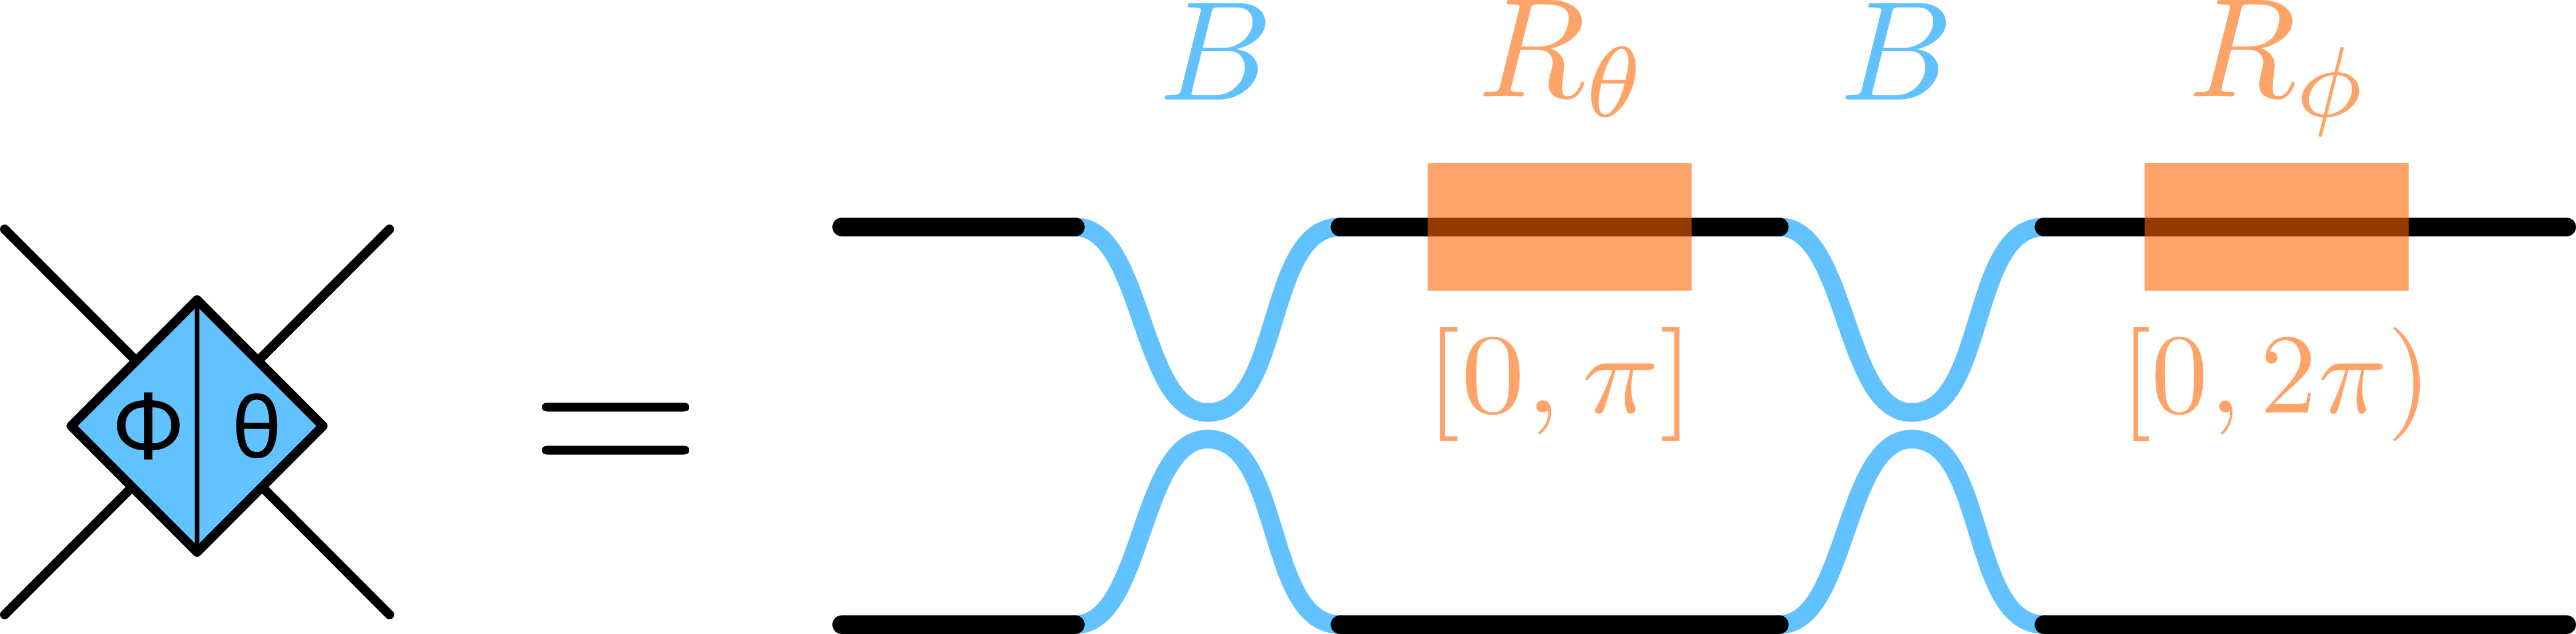
\includegraphics[width=0.5\linewidth]{images/MZISchematics.png}
    \caption{Illustration of a \gls{mzi} composed of beam splitters $B$ and phase shifters $R$. The \gls{mzi} is uniquely characterized by its internal and external phase shift parameters $\theta$ and $\phi$. The black lines represent single mode waveguides, forming the beam splitter using directional coupling.}%nach Miller
    \label{fig:MZI-Phase-shifter}
\end{figure}

%What is training
Training a \gls{nn} means adjusting its parameters such that its predictions match the true result as closely as possible.
This is formalized through a loss function $\mathcal{L}$, which quantifies the discrepancy between the network output and the desired output for a given input.
Training then reduces to a minimization problem: the parameters are iteratively updated along the negative gradient of $\mathcal{L}$ until a minimum is reached.
The practical feasibility of this scheme rests on the backpropagation algorithm \cite{rumelhartLearningRepresentationsBackpropagating1986}.
By applying the chain rule from the output layer backwards, the derivatives with respect to all parameters are obtained in a single pass.
This prevents the cost of a full gradient evaluation from growing with the number of parameters.

%What is Gradient-descent training through physical dynamics
The matrix--vector products required for training can be executed on the physical system itself \cite{hermansTrainableHardwareDynamical2015}. 
Propagating an error field backwards through the device then yields the gradient needed for gradient descent. 
This error field is determined by the deviation of the output from the desired result. 
The central advantage of adjoint-based backpropagation, used in this work, is its scaling~\cite{hughesAdjointMethodInverse2018}. 
The cost of a full gradient evaluation is independent of the number of parameters. 
On hardware, three in-situ intensity measurements after each phase shifter suffice to recover the gradient for all parameters at once. 
Every parameter can then be updated simultaneously to approach a local minimum of the loss landscape. 

The objective of this work is to implement a binary classifier using the \gls{mzi} mesh as the physical core. The model will be trained with samples of handwritten digits ``1'' and ``7'' from the MNIST dataset, using the adjoint-based backpropagation. After the processing layer, two detectors at arbitrary channels will measure the intensity and make a prediction based on the winner-takes-it-all principle. The complete setup is shown in Figure \ref{fig:Objective-Scheme}.
We expect to achieve a high testing accuracy with both the linear regression and the optical model.
In contrast to the linear regression, the optical model has a non-linearity at the detection, which might be an advantage for non-linearly separable problems.
%Expectation?
%The ...
%Und dann kommt noch ein Statement zu den objectives und den expected outcomes
%Objectives: Binäre unterscheidung von handgeschriebenen Ziffern (mnist-dataset)
%(\ref{fig:Objective-Scheme}, MNIST Dataset wird in Vektor zerhackt, geht in input layer, geht durch die Transfer-Matrix, geht in die Detektoren)\\
%Benchmark gegen lineare regression
\begin{figure}[H]
    \centering
    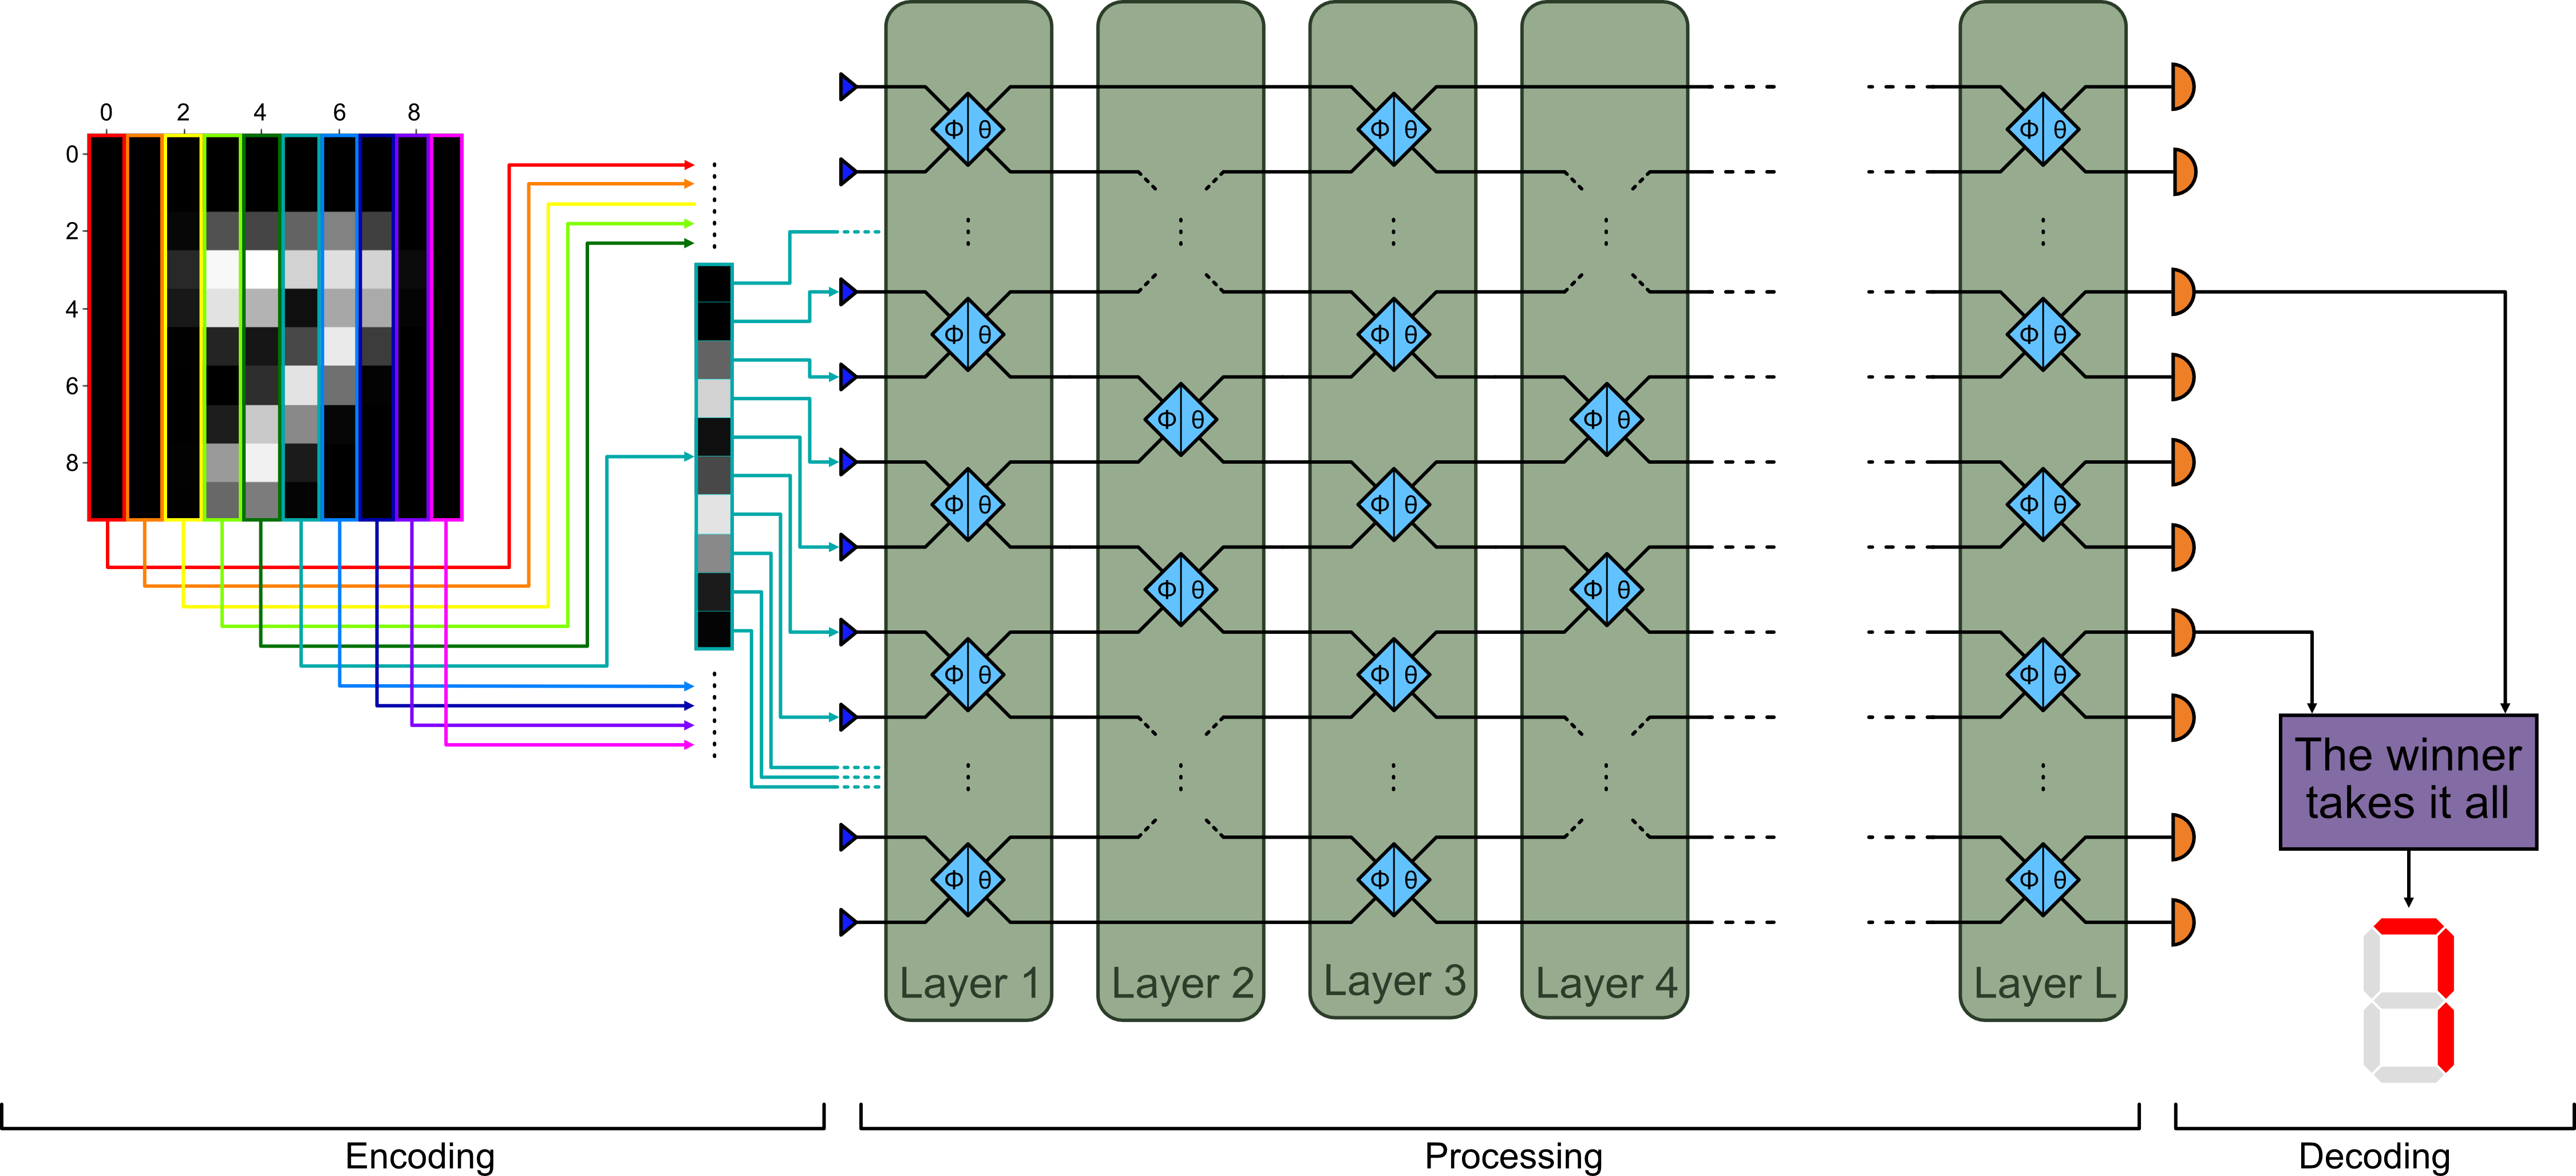
\includegraphics[width=1\linewidth]{images/EncodingProcessingDetectionScheme.png}
    \caption{Scheme illustrating the encoding, processing and decoding steps in the optical model for an image of the MNIST dataset.}
    \label{fig:Objective-Scheme}
\end{figure}
%Expected Outcomes: Mention linear regression, erwarten benefit durch non-linearity am ende (?)
%Außerdem 
%Mention energy-consumption scaling depending on neuron number?
%--> Way more energy-efficient and speed-up

%Vielleicht genauere Einordnung, für welche ML Anwendungen dieser Ansatz gut geeignet ist,... wieso 


%Aus der gegebenen PDF:
%Brief descrip3on of chosen op3cal system and training approach
%Clear statement of objec3ves and expected outcomes
%1 page